
%PREAMBLE
%%%%%%%%%%%%%%%%%%%%%%%%%%%%%%%%%%%%%%%%%%%%%%%%%%%%%%%

\documentclass[titlepage,norsk]{article}
\usepackage{babel,graphicx,amsmath}

\usepackage[utf8]{inputenc}
\usepackage[margin=0.5in]{geometry}


\title{IT3708 - Evolving Spiking-Neuron Parameters}
\author{Odd Andreas Sørsæther \and Andreas Hagen}

%%%%%%%%%%%%%%%%%%%%%%%%%%%%%%%%%%%%%%%%%%%%%%%%%%%%%%%

\begin{document}
\maketitle


\section{System overview}

\paragraph{Our implementation is written in Java. Modularity is handled through ample use of interfaces, employing an architectural strategy influenced by the abstract factory pattern.}

\begin{figure}[h!]
\centering
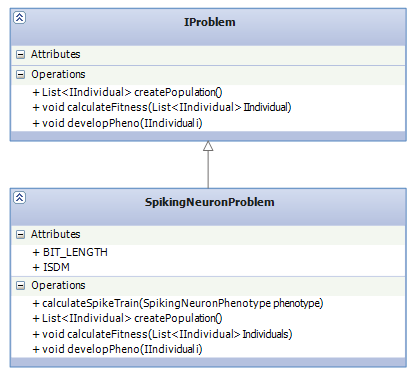
\includegraphics{SpikingNeuronProblem_UML.png}
\caption{UML diagram describing the SpikingNeuronProblem class}
\label{fig:awesome_image}
\end{figure}

\subsection{The Spiking Neuron Problem}

\paragraph{
The heart of this assignment is the class SpikingNeuronProblem which implements the interface IProblem which remains unchanged from Odd Andreas' implementatino of assignment 1. The most important attributes are shown in the class diagram below and are BIT\_LENGTH and ISDM. The ISDM is the distance metric and a description of this interface is given in a later section. The BIT\_LENGTH attribute is the number of bits used to encode the variables a,b,c,d and k in the Izhikevich model. The higher this number, the more decimals can be represented, and the less likely it is that mutations will introduce large changes in the resulting spike train. Through experimentation with the values for the different variables we discovered that the model is extremely sensitive to small changes. Changing the variable by just a small amount can result in a dramatic change in the resulting spike train. In our implementation, we opted for experimenting with values between 15 and 20 bits.
}



\subsection{Spiketrain Distance Metrics}

\paragraph{
The three provided spike distance metrics all implement the interface ISDM (Interface Spike Distance Metric). An SDM is only required to implement the method calculateDistance which takes in two single dimensional arrays that represent the voltage levels of  two different spike-trains where the value at index i represents the voltage level at timestep t+1. The method calculates the distance according to the formulas given and returns a double representing how like each other the two spike trains are. The lower the value, the more they are seen as similar. 
}

\begin{figure}
\centering
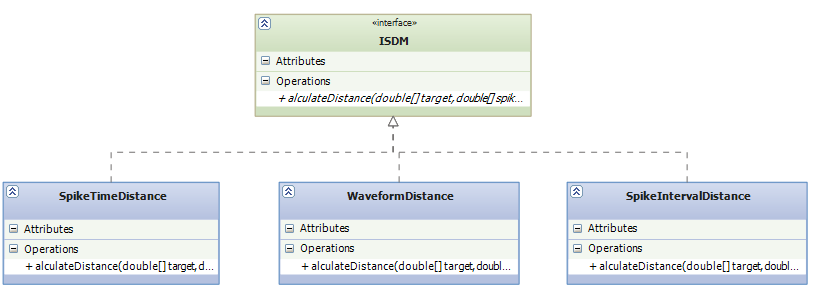
\includegraphics[scale=0.75]{ISDM.png}
\caption{UML diagram describing the ISDM}
\label{fig:awesome_image}
\end{figure}

\subsection{Fitness Function}

\paragraph{
The method calculateFitness calculates fitness for all individuals by first calculating a metric for how dissimilar the phenotype’s spike train is to the target. The largest distance calculated is seen as the worst fitness and is given the value 0. All other fitness values are computed as a percentage of this using \eqref{fitness} where$\phi$ is the fitness, $\delta$ is the current distance being evaluated and $\Delta$ is the largest distance recorded. This means that the fitness function is relative and this entails that a fitness value is not strictly comparable between runs. We have also implemented an optional logarithmic fitness calculation. If logarithmic fitness is chosen, the fitness is calculated using \eqref{logfitness} which causes individuals that have a high distance value to have less impact on the fitness scale.
}

\begin{equation}\label{fitness}
\phi = 1.0 - \frac{ \delta +1.0}{\Delta + 1.0}
\end{equation}


\begin{equation}\label{logfitness}
\phi = 1.0 - \frac{ \log{ ( \delta +1.0 ) } }{\log { ( \Delta + 1.0) } }
\end{equation}

\subsection{Genotype representation}
\paragraph{
The genotype is represented using a very basic bit string. Its size is determined by a hard-coded bit-variable; it symbolizes how many bits is used to represent each variable. Currently our values are encoded in 15 bits, meaning the total genome length is 75. Since the algorithm seems to be incredibly sensitive to minor changes, having a low amount of bits dedicated to each variable (15 bits mean only 32768 possible values) can result in problems when trying to find the exact values used in the target neurons.
Another challenge comes from the fact that the five variables greatly affect the plots in different ways, meaning the EA may easily be misguided. Perhaps an approach more in the style of constraint satisfaction problems would ensure that we could make more informed searches, adjusting only one variable at a time.
}
%%%%%%%%%%%%%%%%%%%%%%%%%%%%%%%%%%%%%%%%%%%%%%%%%%%
%%% GRAPHS'N'SHIT
%%%%%%%%%%%%%%%%%%%%%%%%%%%%%%%%%%%%%%%%%%%%%%%%%%%
\section{Test Case Runs}

\subsection{Izzy Train 1}

\subsubsection{Waveform}

\begin{figure}[h!]
\centering
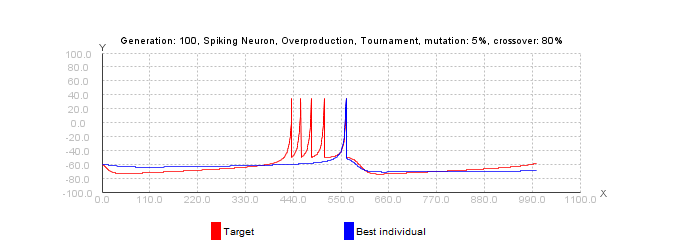
\includegraphics[scale=0.75]{izzy1wave.png}
\caption{Izzy 1 Waveform}
\label{fig:awesome_image}
\end{figure}

\begin{figure}[h!]
\centering
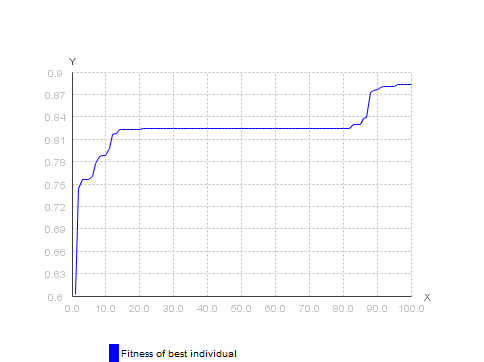
\includegraphics[scale=0.75]{izzy1waveFitness.png}
\caption{Izzy 1 Waveform Fitness Plot}
\label{fig:awesome_image}
\end{figure}

\paragraph{
Generations: 100\\
Population: 100\\
Adult Selection: Overproduction( 50 \%)\\
Selection Method: Tournament (Size: 50, best 10 \%) \\
Mutation : Variable (Initial: 5\%)\\
Crossover: 80\% 1 point split \\
Resulting fitness: 0.86 (logarithmic) \\
Values: a = 0.02, b = 0.265, c = -44.172, d = 5.108, k = 0.041 \\
}

\subparagraph{A symptomatic result using the waveform distance metric. The differences in the graphs at the spikes are not high enough to produce a significant reduction in fitness when averaged out over the entire graph. We experimented with harsher punishment for a difference in spike count, but the results were unimpressing. As is evident from the fitness plot, the EA is prone to getting stuck in local maxima, a recurring problem in our tests. }

\subsubsection{Spike Interval Distance}

\begin{figure}[h!]
\centering
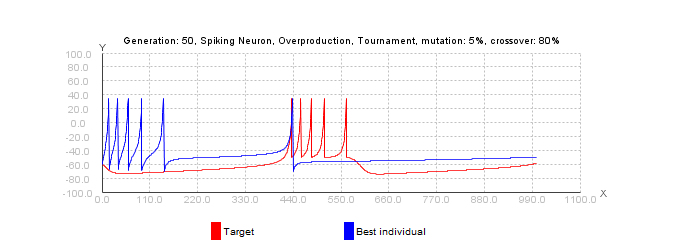
\includegraphics[scale=0.75]{izzy1interval.png}
\caption{Izzy 1 Spike Interval Distance}
\label{fig:awesome_image}
\end{figure}

\begin{figure}[h!]
\centering
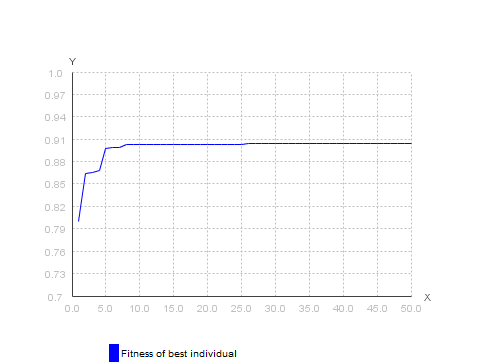
\includegraphics[scale=0.75]{izzy1intervalFitness.png}
\caption{Izzy 1 Spike Interval Fitness Plot}
\label{fig:awesome_image}
\end{figure}

\paragraph{
Generations: 100\\
Population: 100\\
Adult Selection: Overproduction( 50 \%)\\
Selection Method: Tournament (Size: 50, best 10 \%) \\
Mutation : Variable (Initial: 5\%)\\
Crossover: 80\% 1 point split \\
Resulting fitness: 0.90 (logarithmic) \\
 A: 0,002, B: 0,231, C: -74,400, D: 7,166, K: 0,054 \\
}

\subparagraph{This plot is illustrative of the problems with using the spike interval distance metric on this problem. The metric  tends to find the correct shape and then struggles to position it correctly along the time steps. The fitness plot reveals another case of being stuck in a local maxima.}

\subsubsection{Spike Time  Distance}

\begin{figure}[h!]
\centering
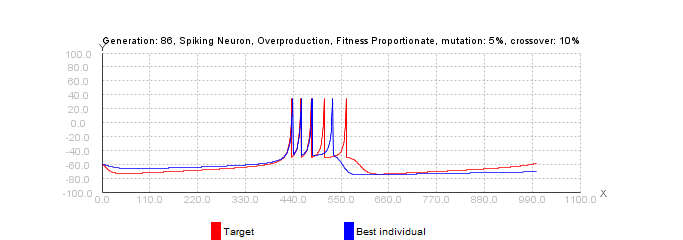
\includegraphics[scale=0.75]{izzy1spike.png}
\caption{Izzy 1 Spike Time Distance}
\label{fig:awesome_image}
\end{figure}

\begin{figure}[h!]
\centering
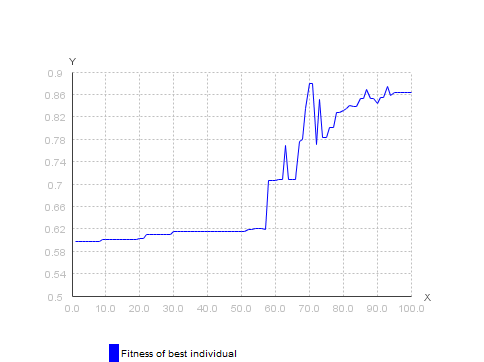
\includegraphics[scale=0.75]{izzy1spikeFitness.png}
\caption{Izzy 1 Spike Time Fitness Plot}
\label{fig:awesome_image}
\end{figure}

\paragraph{
Generations: 100\\
Population size: 100\\
Adult selection: Overproduction (50 \%) \\
Selection method: Fitness proportionate\\
Mutation: Variable,(Initial:  5\% )\\
Crossover: 80\%, 1 point split \\
Resulting fitness: 0.85 (logarithmic) \\
A: 0,007, B: 0,172, C: -47,279, D: 2,821, K: 0,041  \\
}

\subparagraph{A result that is close to what you would expect using the spike time distance metric. The metric  is able to match up the spikes closely, but misses on the number of spikes. Nevertheless, this provides one of the more successful runs and the fitness plot reveals that this run is less plagued with being caught in a local maxima.
}
%%%%%%%%%%%%%%%%%%%%%%%%%%%%%%%%%%%%%%%%%%%%%%%%%%%%%%
\subsection{Izzy Train 2}

\subsubsection{Waveform}

\begin{figure}[h!]
\centering
\includegraphics[scale=0.75]{izzy2wave.png}
\caption{Izzy2 Waveform}
\label{fig:awesome_image}
\end{figure}

\begin{figure}[h!]
\centering
\includegraphics[scale=0.75]{izzy2waveFitness.png}
\caption{Izzy 2 Waveform Fitness Plot}
\label{fig:awesome_image}
\end{figure}

\paragraph{
Generations: 100\\
Population: 200\\
Adult Selection: Full Generational Replacement\\
Selection Method: Tournament (Size: 10, best 30 \%) \\
Mutation : 1+%\\
Crossover: 10\% 1 point split \\
Resulting fitness: 0.83 (logarithmic) \\
 A: 0,003, B: 0,089, C: -50,476, D: 5,829, K: 0,052 \\
}

\subparagraph{The results at the beginning of the spike train are impressive, matching the spikes closely. However, as the spikes move further and further appart, the metric finds that the average distance is sufficient at the bottom, and only produces one spike. The fitness plot again reveals that the EA is stuck in a local maxima.}

\subsubsection{Spike Interval Distance}

\begin{figure}[h!]
\centering
\includegraphics[scale=0.75]{izzy2interval.png}
\caption{Izzy 2 Spike Interval Distance}
\label{fig:awesome_image}
\end{figure}

\begin{figure}[h!]
\centering
\includegraphics[scale=0.75]{izzy2intervalFitness.png}
\caption{Izzy 2 Spike Interval Fitness Plot}
\label{fig:awesome_image}
\end{figure}

\paragraph{
Generations: 100\\
Population size: 100\\
Adult selection: Generational Mixing (20 adult spots) \\
Selection method: Fitness proportionate\\
Mutation:  5\% )\\
Crossover: 80\%, 1 point split \\
Resulting fitness: 0.82 (logarithmic) \\
A: 0,017, B: 0,265, C: -69,485, D: 9,914, K: 0,072 \\
}

\subparagraph{Again we see that spike interval metric manages to create spikes that are distributed in the samme manner as the target graph, but fails to place them correctly. The Fitness plot is more uplifting as the fitness is steadily increasing. However, successive runs with more generations proved less successful.}

\subsubsection{Spike Time  Distance}

\begin{figure}[h!]
\centering
\includegraphics[scale=0.75]{izzy2spike.png}
\caption{Izzy 2 Spike Time Distance}
\label{fig:awesome_image}
\end{figure}

\begin{figure}[h!]
\centering
\includegraphics[scale=0.75]{izzy2spikeFitness.png}
\caption{Izzy 2 Spike Time Fitness Plot}
\label{fig:awesome_image}
\end{figure}

\paragraph{
Generations: 100\\
Population size: 100\\
Adult selection: Generational Mixing (20 adult spots) \\
Selection method: Fitness proportionate\\
Mutation:  5\% )\\
Crossover: 80\%, 1 point split \\
Resulting fitness: 0.87 (logarithmic) \\
A: 0,019, B: 0,281, C: -68,388, D: 4,464, K: 0,047  \\
}

\subparagraph{Here we see behavour that we would expect of spike interval, not spike time, where the spikes are evenly distributed, but not in the correct position and the EA is quickly caught in a local maxima.}


%%%%%%%%%%%%%%%%%%%%%%%%%%%%%%%%%%%%%%%%%%%%%%%%%%%%
\subsection{Izzy Train 3}

\subsubsection{Waveform}

\begin{figure}[h!]
\centering
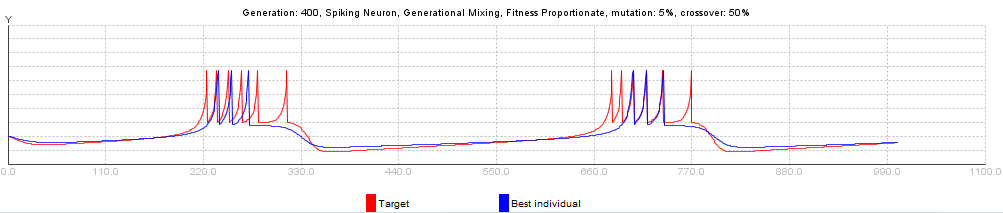
\includegraphics[scale=0.75]{izzy3wave.png}
\caption{Izzy 3 Waveform}
\label{fig:awesome_image}
\end{figure}

\begin{figure}[h!]
\centering
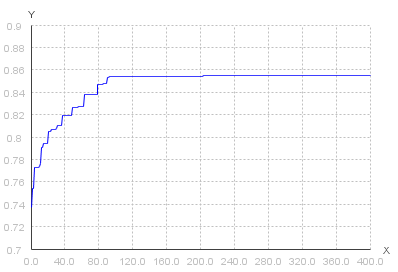
\includegraphics[scale=0.75]{izzy3waveFitness.png}
\caption{Izzy 3 Waveform Fitness Plot}
\label{fig:awesome_image}
\end{figure}

\paragraph{
Generations: 400\\
Population size: 200\\
Adult selection: Generation Mix (10) \\
Selection method: Fitness Proportionate \\
Mutation: 5\% \\
Crossover: 80\%, 1 point split \\
Resulting fitness: 0.88 (logarithmic) \\
Values: a = 0.019, b = 0.14, c = -37.133, d = 5.117, k = 0.041 \\
}
\subparagraph{Here the Waveform SDM shows high fitness after matching a few spikes and  it never seems to find better solutions, or rather other good solutions may not be getting the same fitness levels.}

\subsubsection{Spike Interval Distance}

\begin{figure}[h!]
\centering
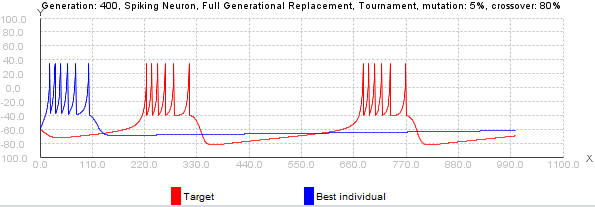
\includegraphics[scale=0.75]{izzy3interval.png}
\caption{Izzy 3 Spike Interval Distance}
\label{fig:awesome_image}
\end{figure}

\begin{figure}[h!]
\centering
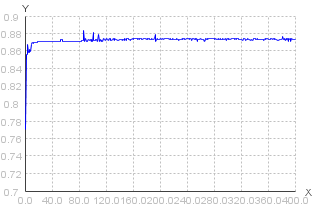
\includegraphics[scale=0.75]{izzy3intervalFitness.png}
\caption{Izzy 3 Spike Interval Fitness Plot}
\label{fig:awesome_image}
\end{figure}

\paragraph{
Generations: 400\\
Population size: 300\\
Adult selection: Full generational replacement \\
Selection method: Tournament (size: 10, best 30 \%) \\
Mutation:  Variable (initial: 5\%), 3 mutations \\
Crossover: 80\%, 1 point split \\
Resulting fitness: 0.87 (logarithmic) \\
Values: a = 0.002, b = 0.23, c = -39.129, d = 5.144, k = 0.047 \\
}

\subparagraph{This plot is symptomatic for Spike Interval on this problem, it tends to find the correct shape and then struggles to position it correctly along the time steps.}

\subsubsection{Spike Time  Distance}

\begin{figure}[h!]
\centering
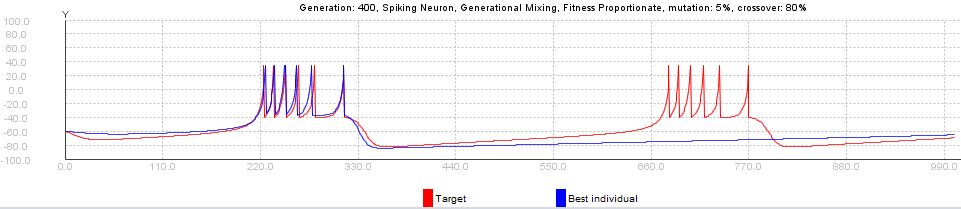
\includegraphics[scale=0.75]{izzy3spike.png}
\caption{Izzy 3 Spike Time Distance}
\label{fig:awesome_image}
\end{figure}

\begin{figure}[h!]
\centering
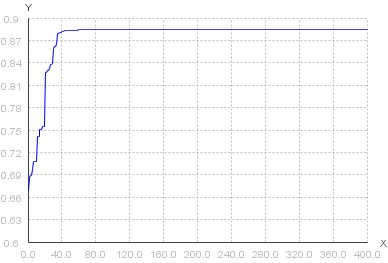
\includegraphics[scale=0.75]{izzy3spikeFitness.png}
\caption{Izzy 3 Spike Time Fitness Plot}
\label{fig:awesome_image}
\end{figure}

\paragraph{
Generations: 400\\
Population size: 200\\
Adult selection: Full generational replacement \\
Selection method: Fitness proportionate\\
Mutation: 5\% \\
Crossover: 80\%, 1 point split \\
Resulting fitness: 0.89 (logarithmic) \\
Values: a = 0.018, b = 0.261, c = -47.92, d = 1.935, k = 0.041 \\
}

\subparagraph{More commonly we get a near-perfect alignment on the first spiking group using spike time and then absolutely no other spikes, but we also tend to get this approximation, which is slightly more interesting.
}

%%%%%%%%%%%%%%%%%%%%%%%%%%%%%%%%%%%%%%%%%%%%%%%%%%%%%%

\subsection{Izzy Train 4}

\subsubsection{Waveform}

\begin{figure}[h!]
\centering
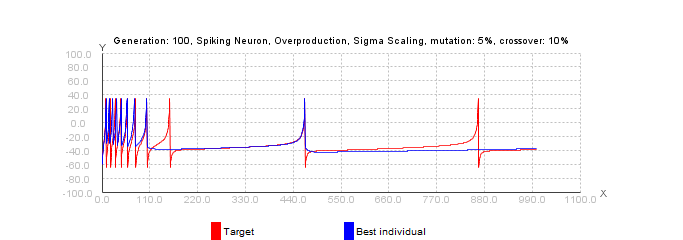
\includegraphics[scale=0.75]{izzy4wave.png}
\caption{Izzy 4 Waveform}
\label{fig:awesome_image}
\end{figure}

\begin{figure}[h!]
\centering
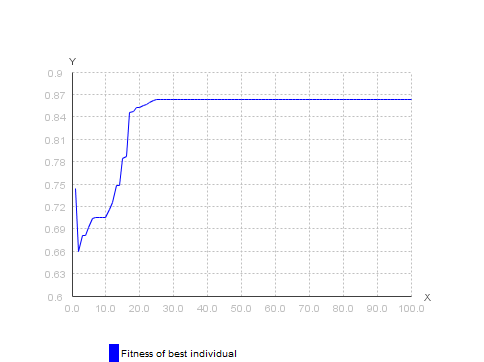
\includegraphics[scale=0.75]{izzy4waveFitness.png}
\caption{Izzy 4 Waveform Fitness Plot}
\label{fig:awesome_image}
\end{figure}

\paragraph{
Generations: 100\\
Population: 200\\
Adult Selection: Overproduction( 50 \%)\\
Selection Method: Sigma Scaling \\
Mutation : Variable (Initial: 5\%)\\
Crossover: 10\% 1 point split \\
Resulting fitness: 0.86 (logarithmic) \\
Values:A: 0,001, B: 0,173, C: -35,664, D: 8,867, K: 0,076 \\
}

\subparagraph{As before, the waveform SDM is able to match the spikes where they are closed together, but misses the two of the spikes because it is pleased with the average distance as the best individual hugs the graph closely at the bottom.}

\subsubsection{Spike Interval Distance}

\begin{figure}[h!]
\centering
\includegraphics[scale=0.75]{izzy4interval.png}
\caption{Izzy 4 Spike Interval Distance}
\label{fig:awesome_image}
\end{figure}

\begin{figure}[h!]
\centering
\includegraphics[scale=0.75]{izzy4intervalFitness.png}
\caption{Izzy 4 Spike Interval Fitness Plot}
\label{fig:awesome_image}
\end{figure}

\paragraph{
Generations: 100\\
Population: 200v\\
Adult Selection: Overproduction( 50 \%)\\
Selection Method: Fitness Proportionate \\
Mutation : Variable (Initial: 5\%)\\
Crossover: 10\% 1 point split \\
Resulting fitness: 0.91 (logarithmic) \\
A: 0,010, B: 0,194, C: -34,295, D: 5,167, K: 0,044 \\
}

\subparagraph{An interesting case where yet again the spacing is matched, but not the position. The EA fails to match the spacing of the last three spikes, but has a high fitness value. This reveals some of the problems you would expect when using relative fitness.  }

\subsubsection{Spike Time  Distance}

\begin{figure}[h!]
\centering
\includegraphics[scale=0.75]{izzy4spike.png}
\caption{Izzy 4 Spike Time Distance}
\label{fig:awesome_image}
\end{figure}

\begin{figure}[h!]
\centering
\includegraphics[scale=0.75]{izzy4spikeFitness.png}
\caption{Izzy 4 Spike Time Fitness Plot}
\label{fig:awesome_image}
\end{figure}

\paragraph{
Generations: 100\\
Population size: 200\\
Adult selection: Full Generational Replacement \\
Selection method: Fitness proportionate\\
Mutation: Variable,(Initial:  5\% )\\
Crossover: 10\%, 1 point split \\
Resulting fitness: 0.88 (logarithmic) \\
 A: 0,002, B: 0,205, C: -40,516, D: 7,559, K: 0,067  \\
}

\subparagraph{In using the full generational replacement, a fairly good solution is found, but as is evident from the fitness plot, it is soon lost as small variations in the genome can produce large variations in the resulting graph. By using full generational replacement we avoid the problem with local maximas, but since the phenotypes are so suceptible to small changes in the genome it only takes a few crossovers and mutation before an entire generation of good solutions evolves into poorer ones.
}

%%%%%%%%%%%%%%%%%%%%%%%%%%%%%%%%%%%%%%%%%%%%%%%%%%%
%%%END OF GRAPHS'N'SHIT
%%%%%%%%%%%%%%%%%%%%%%%%%%%%%%%%%%%%%%%%%%%%%%%%%%%

\section{Classification of genotype-to-phenotype mapping}
\paragraph{Syntactically, the genotype is a fixed length linear object, and semantically the genotype is data oriented. The encoding scheme is a generative one, since the genes encode the vaules of variables in an equation, and thus the appearance of the phenotype is not only directly related to the values encoded in the genotype, but is dependent on how the phenotype is developed.}

\section{Practical Implications of the Implementation}
\paragraph{The algorithm is designed to match target values and a neuroscientist who is able to record the voltage in a neuron when it fires could use the algorithm to determine the weights that produce the particular spike train. This again could be used to map out how a section of a real neural network respongs to input, in particular how the weights change when the soma is stimulated repeatedly.}
\section{Other Problem Domains}

\paragraph{
One could create an ensemble of evolutionary algorithms using specialization-variants of this problem to find mathematical functions that fit a set of values, in other words, the EA could be easily modified to host a set of general curve fitting algorithms.The algorithms could compete against each other and the EA that produces the best fitness value (best matching the plots) will be chosen. There could for instance be EAs for exponential functions, logarithmic functions, etc. 
}



\end{document}